\chapter{Path Finding for Multiple Robots}\label{sec:app}

%Although the main focus of this chapter is the \textsc{Area Protection Problem} APP, 
%we first provide and overview of relevant problems  \textsc{Multi-Agent Path Finding} (MPF) and its variants before pursuing APP itself because APP shares many features wih other modifications of MPF, 
%and it is therefore more natural to introduce the simpler variants earlier.

Before focusing on path finding for multiple robots, let us summarize techniques for simple path finding in graphs, which act as building blocks in environments with multiple robots.

\section{Basic Path Finding}

Basic path finding is a well known task in computer science.
Given a graph $G=(V,E)$, the objective is to find a path between two selected points $s$ and $t$ referred to as  \emph{source} and \emph{target}, respectively.
Graph searching methods such as breadth-first search and depth-first search find a path if given a sufficient amount of time. 

The aim is often to find a shortest path between source and target in $G$ with given edge costs.
Exhaustive search examining all possible paths employed in Bellman-Ford algorithm yields a shortest path in $\mathcal{O}(|V||E|)$.

A common approach used for finding a shortest path is \emph{Dijkstra's algorithm} \cite{dijkstra59}, which guarantees to yield an optimal path in $\mathcal{O}(|E|\log|V|)$ time.
Dijkstra’s Algorithm visits vertices in the graph starting with the source. 
It then repeatedly inspects the vertex which was not yet visited that lies closest to the source. 
It expands outwards from the source until it reaches the target. 
A drawback of this approach is that it may expand too many vertices that later turn out to lie very far from the target.

Another possibility is the greedy \emph{best first search} algorithm which can find the target faster, but the selected path is not guaranteed to be optimal.
Instead of expanding vertices close to the source, it selects those close to the target.
Obviously, which node is exactly the closest is not known without a previous preprocessing, and so it uses a heuristic estimation which guides the way towards the target.

The \emph{A*} algorithm \cite{hart68} combines the advantages of Dijkstra's and best first search algorithm.
It guarantees to find an optimal path and also exploits a heuristic estimation of the distance to the target, which helps to avoid expanding unsuitable vertices.
The heuristic estimation is particularly useful when there is an incomplete information of the graph.
For that reason, A* is popular in video game development, where the exact distances can not be predicted due to a frequent change of the environment, 
or due to a lack of knowledge of the current situation in the environment.

A* searches a shortest path from $s$ to $t$ by maintaining a tree of paths originating at $s$, and extending those paths until its termination criterion is satisfied.
Alg.~\ref{alg:astar} shows a pseudocode of A*.
At each iteration, the algorithm determines which of its paths should be extend. 
The selection is based on the cost of the path so far and a heuristic estimate of the cost required to extend the path all the way to $t$. 
Specifically, A* chooses the path that minimizes
$$
    f(v)=g(v)+h(v),
$$
where $v$ is the node by which the path is extended, $g(n)$ is the cost of the path from the $s$ to $v$, 
and $h(n)$ is the heuristic estimation of the cost of the cheapest path from $v$ to the target $t$. 
A* terminates when the path it chooses to extend is a path from start to goal or if there are no paths eligible to be extended.

The performance of A* strongly depends on the selected heuristic function $h$.
The heuristic is \emph{admissible} if $h(v)\leq$ the shortest path from $v$ to $t$.
An admissible heuristic is an optimistic estimation as it considers a shorter path than it actually is. 
Thus, $f(v)$ is a lower bound on the path cost via $v$.
The heuristic is said to be \emph{monotonous} or \emph{consistent} if for some $v'\in N(v)$ we have that $h(v)\leq w_{vv'}+h(v')$.
\begin{observation}
Every monotonous heuristics is admissible.
\end{observation}
\begin{proof}
Let $s=v_1,v_2,\dots,v_k=t$ be an optimal path.
As $h$ is monotonous, we have that $h(v_i)-h(v_{i+1})\leq w_{v_iv_{i+1}}$.
	This implies that $h(v_1)\leq\sum_{i=1}^{k-1}w_{v_iv_{i+1}}$.
\end{proof}
\begin{observation}
For a monotonous heuristic, the values of $f(n)$ are not decreasing along any path.
\end{observation}
\begin{proof}\label{obs:monnondec}
	Let $v'\in N(v)$, i.e., $g(v')=g(v)+w_{vv'}$.
Then, $f(v')=g(v')+h(v')=g(v)+w_{vv'}+h(v')\geq g(v)+h(v)=f(v)$.
\end{proof}
\begin{proposition}
If $h$ is a monotonous heuristic, A* finds an optimal path.
\end{proposition}
\begin{proof}
	A* selects for expansion the node $v$ with minimal value of $f$ 
	By Obs.~\ref{obs:monnondec}, if $h$ is monotonous, the values of $f(v)$ are not decreasing along any path.
	Thus, the path selected from $s$ to $v$ is optimal, which is inductively extended up to $t$.
\end{proof}
If the trivial monotonous heuristic $h(v)=0$ for all $v\in V$ is used, the algorithms becomes Dijkstra's algorithm.

\begin{algorithm}
\DontPrintSemicolon
\SetAlgoLined
%\KwResult{Write here the result}
\caption{A* algorithm}
\BlankLine
\SetKwInOut{Input}{Input}\SetKwInOut{Output}{Output}
\Input{$G=(V,E)$, $s,t\in V$, $w: E\mapsto\mathbb{R}^+$}
%\Output{Write here the output}
\BlankLine
$C\leftarrow\emptyset$\;
$O\leftarrow\left\{s\right\}$\;
\For{$v\in V\setminus\left\{s\right\}$} {
	$g(v)\leftarrow\infty$\;
	$f(v)\leftarrow\infty$\;
}
$g(s)\leftarrow 0$\;
$f(s)\leftarrow h(s)$\;
\While {$O\neq\emptyset$}{
	$v\leftarrow$ select a node from $\arg\min\left\{f(u):u\in O\right\}$\;
	\textbf{if }{$v=t$}\textbf{ then return } path from $s$ to $t$ reconstructed using $\pi$\;
	$O\leftarrow O\setminus\left\{v\right\}$\;
	$C\leftarrow C\cup\left\{v\right\}$\;
	\For{$u \in N(v)$} {
		\textbf{if }{$u\in C$}\textbf{ then continue}\;
		$tmp\leftarrow g(v) + w_{v,u}$\;
		\textbf{if }$u\not\in O$ \textbf{ then } $O\leftarrow O\cup\left\{u\right\}$\textbf{ else if }{$tmp\geq g(u)$}\textbf{ then continue}\;
		$\pi(u)\leftarrow v$\;
		$g(u)\leftarrow tmp$\;
		$f(u)\leftarrow g(u)+ h(u)$\;
	}
} 
\textbf{return } failure
\label{alg:astar}
\end{algorithm}

These are two different perspectives of the running time. 
The first way counts the running time as a function of $|V|$ and $|E|$, which is more common in the context of graph theory.
In this case, if the monotonous heuristic is determined in a constant time, the complexity of A* equals the complexity of Dijkstra's algorithm. 
Another way popular in AI community is measuring the running time in terms of a depth of a solution and a branching factor.
In this context, graphs are typically very large, and avoiding to examine the entire graph is desirable, in fact, it is one of the major goals of the algorithm.
If we examine every node at depth up to $d$ before the target is found, we end up visiting $\mathcal{O}(b^d)$ nodes before termination.
\section{Path Finding for Multiple Robots}

The requirement of finding multiple non-colliding paths significantly increases the complexity of the problem.

We consider an environment with several identical moving entities referred to as \emph{agents}. 
Source and target locations are uniquely determined for each agent. 
The objective is to find a route for every agent from its source to its target while avoiding obstacles in the environment..
The environment is modeled as an undirected graph, where the agents are placed in the nodes, and move along the edges from one node to another. 
In this context, the paths/routes are allowed to contain a node multiple times.
Movement of the agents is carried out in discrete time steps, where the relocation of an agent from one node to its neighbor takes exactly 1 time step.
Agents must not collide with obstacles and other agents that are also moving along planned routes towards their own targets.

Methods for solving MPF are divided into two main approaches: \emph{centralized (coupled)} and \emph{decentralized (decoupled)}.
A centralized approach incorporates a global decision maker that regards all the agents as a single entity, and plans paths for them simultaneously.
On the other hand, a decentralised approach can considerably reduce computations by decomposing the problem into several smaller subtasks.
Paths are typically computed for each agent individually, ignoring all other agents.
The interactions are handled along the way to avoid collisions.
This is usually much faster but yields suboptimal solutions and loses completeness \cite{ryan08}.

LRA* \cite{silver05} is a decentralized algorithm readily applicable to MPF.
Each  agent searches for a route to the destination using the A* algorithm, ignoring all other agents except for its current neighbours. 
The agents then start to follow their routes, until a collision is impending.  
Whenever an agent is about to move into a position occupied by another agent, it instead replans the route from its current position.

Problems dealing with navigating a group of mobile robots can be formulated as multi-agent pat planning.  
However, the primary motivations for the problem are tasks of moving certain entities within an environment with obstacles.
The constraint of limited free space represents a key aspect that makes the problem non-trivial. 
Examples of applications include: 
Parcel delivery in office building by multiple mobile robots \cite{hada01},
navigation of robots within an industrial warehouse environment \cite{everett95},
control and the management of a fleet of autonomous mobile robots for transshipment tasks in harbors, airports and marshalling yards \cite{alami98}.
Shipping container rearranging can also be formulated as path-planning for multiple agents where agents are represented by containers \cite{surynek11}.

\subsection{Mathematical model and variants}\label{sect:modvar}

The problem of path finding for multiple robots is defined by a quadruple $(G,R,\lambda_0,\lambda_+)$, where
\begin{enumerate}
	\item $G=(V,E)$ is an undirected graph representing the environment,
	\item $R=\left\{r_1,\dots,r_{|R|}\right\}$ is the set of robots or agents, $|R|\leq|V|$,
	\item $\lambda_0:R\mapsto V$ is an injective function that assigns each agent its initial node, and
	\item $\lambda_+:R\mapsto V$ denotes an injective function that assigns a target node to each agent.
\end{enumerate}
In general, there is no restriction on the graph, but majority of works in this area considers 4 or 8-connected grid graphs with some missing nodes representing obstacles.
There are the following two different models of dynamics of the movement: \emph{Multi-Agent Path Finding} (MPF) and \emph{Pebble Motion on Graph} (PMG).

\paragraph{Multi-Agent Path Finding}
An agent can shift from one node to its neighbor on condition that the neighbor is either unoccupied or is being left by other agent in the same time step. 
At most one agent is allowed to pass an edge within one time step. 
That is, agents are not allowed to exchange their positions within one time step.
Finally, no two agents can enter the same node at the same time, as there cannot be more than one agent simultaneously at a node.
Under this settings, the optimization variant of MPF was shown to be NP-hard \cite{surynek10}.

In general, agents are considered as independent isolated units, and one agent is not aware of other agents' path plans.
There are variants of MPF where this is not the case (see Sect.~\ref{sec:cpf}).

\paragraph{Pebble Motion on Graphs}
\emph{Pebble motion on graphs} \cite{kornhauser84} can be regarded as a restricted variant of MPF. 
The difference consists in rules for movement. 
While MPF enables entering a vertex that is simultaneously being left by other agent, such transfer is not permissible in pebble motion. 
Thus, the restriction of movement in pebble motion is that only one agent is allowed to move in each time step.
As an illustration we mention the 15-puzzle also known as Lloyd’s 15 \cite{archer99}.
Its generalized $N\times N$ version has been proved to be NP-hard in \cite{ratner86}.  
The situation becomes much easier when the optimality of the number of moves, i.e., when the problem is to find any sequence of movement so that the target locations are reached.
In this case the problem belongs to $P$ \cite{kornhauser84}, and so is MPF when optimality is abandoned, as every solution to PMG is a solution to MPF.
As all results relevant to this chapter consider the movement rules of MPF, PMG is not discussed any further.

There are three most common optimization criteria \cite{yu13} to be pursued:
\begin{itemize}
        \item Minimum total arrival time - total number of time steps that the agents need before arriving in their targets.
        \item Minimum makespan - the number of time steps needed by the latest arriving agent.
        \item Minimum total distance - total number of moves performed by the agents.
\end{itemize}
In a corresponding decision problem, we are given a parameter $k$ and ask whether it is possible that agents reach their targets so that the objective function does not exceed $k$.
\subsection{Cooperative Path-Finding}\label{sec:cpf}

\emph{Cooperative Path-finding} \cite{silver05} is a special case of MPF where each agent is assumed to have a full knowledge of all other agents and their planned routes.
Precisely speaking, solving algorithm can take into account paths planned for agents that were processed earlier, and adjust paths searched later according to them.
The concept of CPF is most relevant to the contribution of this thesis, as all the studied variants assume a knowledge of at least some agents' path planning.

\subsubsection{CA*}

A decoupled algorithm for solving CPF known as cooperative A* (CA*) has been introduced in \cite{silver05} together with several improvements reducing its complexity.
Its basic version works with a \emph{spatial graph} $G'$ constructed from the initial graph $G=(V, E)$.
The spatial graph can be regarded as $k$ copies (layers) $G_0, G_1,\dots,G_k$ of $G$, which are arranged parallel with each other.
These layers represent the time dimension of the agents' movement.
All edges within one layer are removed, because a movement along them would represent an agent's change of position in zero time, which is prohibited by the rules for movement.
Consider nodes $v_i$ and $v_{i+1}$ in two consecutive layers of $G'$, both corresponding to node $v$ in the origianal graph.
Further, let $v_{i+1}^1,\dots v_{i+1}^{|N(v)|}$ be the nodes in the $(i+1)$-th layer corresponding to neighbors of $v$ in the original graph.
The spatial graph contains edge $\left\{v_i,v_{i+1}\right\}$, which represents an agent staying at its node from time step $i$ to $i+1$, 
and edges $\left\{v_i,v_{i+1}^{1}\right\},\dots,\left\{v_i,v_{i+1}^{|N(v)|}\right\}$ representing an agent's movement to the adjacent nodes.
Edges in $G'$ are always directed from the lower layer to the higher layer, as it is forbidden to move ``back in time''.

Agents are initially placed in the first layer of $G'$, and if a node $t$ is a target of some agent $a$ in the original graph, nodes corresponding to $t$ in each layer become targets of $a$ in $G'$,
and $a$ must reach one of them.
This models the fact that an agent can reach its target at any time step.
The algorithm processes agents one by one, and always searches a path in $G'$ for a currently considered agent using A*.
Once a path is found in $G'$, its nodes in $G'$ are \emph{reserved}, and agents processed afterwards must avoid the reserved nodes.

CA* is neither complete, nor optimal. It is however popular because it does not pose any specific requirement on the instance and also because of its simplicity.
An example of an instance for which CA* is unable to find a solution is depicted in Fig.~\ref{fig:castarfail}.
\begin{figure}
\centering
	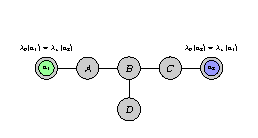
\includegraphics[scale=1.5]{figurer/castarfail.eps}
\caption{An instance for which CA* fails to find a solution}
\label{fig:castarfail}
\end{figure}
The instance consists of a path on five nodes and a node adjacent to the central node of the path.
Agents $a_1$ and $a_2$ are placed at the two endpoints of the path, and have targets $t_1$ and $t_2$, respectively.
This instance has a solution in which one agent uses the node outside of the path in order to allow the other agent to pass towards its target.
%It does not matter which agent is considered first by the algorithm, so let us assume $a_1$ is processed first.
CA* finds a path in the spatial graph that corresponds to the shortest path from $a_1$'s initial position to $t_1$, and when $a_2$ is processed,
a path to $t_2$ in $G'$ that avoid reserved nodes does not exist.
If there was another node between $t_2$ and the central node of the path, the solution would have been found by CA*, in which agent $a_2$ makes a step aside so that the two agents can pass each other.

The quality of a solution often depends on the order in which agents are processed. 
In some ordering of agents, a solution may not exist, while there can be a solution for another ordering.

\subsubsection{OD+ID}

An example of a coupled algorithm is to apply A* on the following state space:
Each state is encoded as an $|R|$-tuple representing all agents' positions.
There is an edge between two states if and only if the transition between the two states represents a valid move.
With this representation, A* finds an optimal solution, but the obvious drawback of this approach is its time and space complexity.
The size of the state space is $\mathcal{O}(|V|^{|R|})$ with the branching factor $\mathcal{O}(d_{max}^{|R|})$ where $d_{max}$ is the maximum degree in $G$.

An improvement of this naive approach is achieved by \emph{operator decomposition} (OD)\cite{standley10}.
In this approach, a fixed ordering of agents is assumed, and a move is assigned to each agent in succession.
Thus, a transition from one state to another corresponds to  moving only one agents while other agents' positions remain unchanged.
Under this representation, every $|R|$-th state corresponds to a full move of the group of agents, and is known as \emph{standard state}. 
The other states are referred to as \emph{intermediate states}.
Standard and intermediate states are conceptually different, they are nevertheless treated equivalently by A*.

Although operator decomposition allows the algorithm to avoid considering a substantial portion of the search space, the resulting algorithm is still exponential in the number of agents \cite{standley10}.
Independence detection (ID) aims to plan a path for agents as independently as possible.
The idea is to plan paths for agents separately whenever a cooperation is not needed as they would not collide if they moved along their shortest paths.
When OD is combined with ID, agents are divided into groups which are then planned separately using OD.
Once a plan for all groups is known, the movement is simulated, and if the plans for two or more groups contain conflicts,
the affected groups are merged together, and a new plan is searched for these larger groups.

\subsubsection{Other notable algorithms}

Besides the methods described above, there are many algorithms of various properties designed for CPF in recent decades, and the research in this area still continues. 

An alternative method developed in \cite{jansen08} achieves an implicit cooperation among agents by using so called direction maps.

In \cite{wang08}, a decoupled algorithm \emph{flow annotated replanning} FAR for grid graphs is presented.
FAR trades the completeness for an improved efficiency, and uses an abstraction of the grid graph into a flow-annotated grid graph.
A* is then applied separately for each agent in this abstracted environment.

Another CPF algorithm that claims completeness is \emph{Push and Swap} \cite{luna11}. 
However, in \cite{wilde13} were identified instances for which this algorithm fails to obtain a solution.
Consequently, algorithm \emph{Push and Rotate} is then presented as an adaptation of the Push and Swap technique. 
By fixing the Push and Swap’s shortcomings, the authors developed an algorithm that is complete for the class of instances that contain at least two unoccupied nodes.

\section{Scenarios with adversaries}

Consider a problem of MPF where agents are divided into two (or more) adversarial teams competing for achieving some goal.
The teams move in turns so that the $i$-th team moves in every $i$-th time step, while agents of other teams act as obstacles.

The division into adversarial team is a generalization of MPF that increases the problem's complexity.
The problem becomes a two-player game with full information, and so various search space algorithms developed for these types of games are applicable for adversarial versions of MPF.
Examples of these algorithms are alpha-beta algorithm widely applied on computer chess, or Monte Carlo tree search which were recently successfully employed in the game of Go.
These algorithms are often combined with methods of machine learning such as neural networks and genetic algorithms.

In problems with adversarial element, we consider one specific team of agents, and try to solve the decision problem whether there exists a winning strategy for the selected team. 

\subsection{Adversarial Cooperative Path Finding}

In \textsc{Adversarial Cooperative Path Finding} (ACPF), all the agents are defined by their initial and target node in a graph, 
and the task of one team is to reach all the targets by corresponding agents before the opponent's agents reach their positions.
In general, it is not required that the teams are of the same size, although it is typically assumed that the teams are of equal number of agents.
Similarly, the placement of targets of the teams does not have to be symmetric, and so the starting condition are not necessarily ``fair'' for the teams.

Besides the points 1.-4. in Sect~\ref{sect:modvar}, the formal definition consists of the following elements:
\begin{enumerate}
		\setcounter{enumi}{4}
	\item $\mathcal{T}=\left\{T_1,T_2,\dots,T_{|\mathcal{T}|}\right\}$, $|\mathcal{T}|\leq|R|$ contains the set of disjoint teams.
		Each agent belongs to exactly one team. 
		Two teams are considered in a typical instance. 
	\item $t^*\in\left\{1,2,\dots,|\mathcal{T}|\right\}$ denotes the index of a team for which the strategy is searched, 
		and for which the answer whether there exists a winning strategy is of interest.
\end{enumerate}
It is also assumed that there is a mechanism that determines the next move of a team different from $T_{t^*}$ when given the sequence of all agents' previous placements. 
This mechanism is unknown, and is expected to act as an oracle that is able to determine the best possible move for an adversarial team in each time step.
\begin{problem}
Given an instance $(G,R,\lambda_0,\lambda_+,\mathcal{T},t^*)$, is it possible to determine the movement of team $T_{t^*}$ at every time step in which the team is to move 
so that every agent $a\in T_{t^*}$ reaches its target location $\lambda_+(a)$, and so that no other team reaches its desired locations earlier?
\end{problem}

The problem was proved to be PSPACE-hard for two teams in \cite{ivanova04} by a polynomial reduction from \textsc{Quantified Boolean Formula} (QBF).
It is also known that the problem is EXPTIME, but Whether or not it belongs to PSPACE remains an open question.

In experimental settings, a time limit during which the agents move is imposed.
When this limit is up, the winner is the team whose agents captured the highest number of target nodes.

\subsection{Area Protection Problem}

Another concept of adversarial MPF is the \textsc{Area Protection Problem} (APP), where two teams of agents compete in reaching their target positions. 
Unlike ACPF, where the goals of both teams of agents is to reach their targets, the adversarial teams in APP have different objectives. 
The first team of \emph{attackers} consists of agents whose goal is to capture a pre-defined targets in the area protected by the second team of \emph{defenders}. 
There is a one-to-one mapping between attackers and target nodes.
The opponent team of defenders aims to prevent the attackers from reaching their targets by occupying selected locations.

The common feature in all MPF problems is that once a location is occupied by an agent, 
it cannot be entered by another agent unless it is first vacated by the agent which occupies it (agents cannot push away each other). 
This property is a key tool for the team of defenders.
Formally, the problem is defined using points 1.-3. in Sect.~\ref{sect:modvar}, and
\begin{enumerate}
	\setcounter{enumi}{4}
	\item $D\subseteq R$ and $A\subseteq R$ with $D\cap A=\emptyset$ and $D\cup A=R$, that is, an agent is either attacker or defender,
		Each agent belongs to exactly one team. 
		Two teams are considered in a typical instance. 
	\item $\lambda_+^A:A\mapsto V$, an injective function that assigns a target node to each attacker.
\end{enumerate}

Defenders do not have any pre-defined targets, as their objective is to prevent attackers from reaching their targets.
The decision version of APP is formulated as 
\begin{problem}\label{prob:app}
	Given an instance $(G,R,\lambda_0,A, D, \lambda_+^A)$, is it possible to navigate the defenders in a way that no attacker reaches its target?
\end{problem}
Paper V \cite{ivanova18a} contains a PSPACE-hardness proof of APP.
%The formulation of Prob.~\ref{prob:app} has mainly a theoretical relevance, as most of the instances 

Like in problems without the adversarial element, there are several possible objective functions of APP:
\begin{itemize}
        \item Maximize the number of targets not captured by attackers.
        \item Maximize the sum of distances between attackers and their targets.
        \item Minimize the time spent by attackers at captured targets.
\end{itemize}
The available literature focuses on the first objective.

\subsection{Area Protection Problem with Communication maintenance}

An extension APP by a requirement of communication maintenance (APPC) has been introduced in Paper VI \cite{ivanova18b}.
The environment is assumed to be a 4-connected grid graph with possible missing nodes (obstacles), which allows to define the connectivity constraints.

Graph $G$ is embedded in a plane so that all edges have length 1 unit and each node $v$ has coordinates $(x_v,y_v)$.
The physical location $l_v$ represented by $v$ is the unit square centered at $C_v=(x_v,y_v)$.
Further, the set $B$ consists of square areas representing obstacles.
The visibility range $r$ is the maximum distance between two locations between which the communication can be established.
A communication is impossible between locations $l_u$ and $l_v$ if the line segment $C_uC_v$ intersect any obstacle. 
\begin{definition}
	Given a visibility range $r$, $G_r=(V,E_r)$ where \newline
	$E_r=\left\{\left\{u,v\right\}:C_uC_v\cap B=\emptyset\text{ and } |C_uC_v|\leq r\right\}$ is the visibility graph of $G$.
\end{definition}

The decision problem is derived from Prob.~\ref{prob:app} with the additional requirement of connectivity formulated as
\begin{problem}
	Let $S_t\subseteq V$ be the set of nodes occupied by defenders at time step $t$.
	Given an instance $(G,R,\lambda_0,A, D, \lambda_+^A)$, is it possible to navigate the defenders in a way that no attacker reaches its target,
	and the induced subgraph $G_r\left[S_t\right]$ of the connectivity graph remains connected at every time step?
\end{problem}
NP-hardness of APP implies also the same result for APPC.
